\chapter{Fundamentação e Trabalhos Relacionados}
\label{cap:fundamentacao}
Este capítulo está estruturado em duas seções, a primeira apresenta os conceitos necessários para o entendimento desse trabalho. A segunda apresenta os trabalhos que estão relacionados à correspondência de instância.

\section{Fundamentação Teórica}
O objetivo desta seção é apresentar a fundamentação teórica referente ao foco deste trabalho, fazendo uma pequena introdução  sobre conceitos da área que auxiliam na compreensão da pesquisa desenvolvida.

\subsection{RDF (Resource Description Framework)}

RDF trata-se de um \textit{framework} de descrição de recursos, trabalhando como um alicerce para a construção de Dados Conectados. Em concordância com tecnologias Web, bem como Dados Conectados, o modelo RDF utiliza URIs para identificação de recursos, permitindo que os recursos sejam descritos uniformemente na Web. Basicamente, o RDF é estruturado em triplas do tipo sujeito, predicado, objeto (ver Figura \ref{fig:spo}). 

\begin{figure}[!ht]
	\centering
	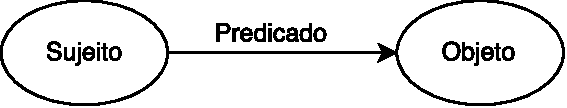
\includegraphics[width=0.5\textwidth]{./imagens/Sujeito-predicado-objeto.pdf}
    \caption{Estrutura da tripla RDF}
%	\footnotesize{Fonte: Próprio autor.}
	\label{fig:spo}
\end{figure}

A estrutura do RDF pode se materializar de várias formas. Cada uma dessas formas recebe o nome de serialização RDF. Atualmente existe um conjunto considerável de serializações tais como: RDF/XML, Turtle, N-Triples e outros. Onde cada serialização tem um uso em potencial. Por exemplo, Turtle é usado para ser lido por humanos, pois ele é melhor estruturado para isso. 

Vale a pena salientar que RDF é um framework de descrição, não sendo responsável por atribuir semântica aos recursos descritos, sendo as ontologias responsáveis por esta função. Por esta razão, um número considerável de processos de publicação de Dados Conectados \cite{bizer2007publish, hyland2011joy, villazon2011methodological, Avila2015} recomenda o reuso de ontologias. 

\subsection{Ontologias}
Os Dados Conectados fazem uso de ontologias como suporte formal para representação de conhecimento, pois só RDF não é o bastante para que máquinas consigam entender a relação entre os dados. Desta forma, as ontologias têm um papel fundamental na modelagem e descrição de dados. A palavra ontologia vem do Grego \textit{ontos} e \textit{logos}, significando conhecimento do ser. Em filosofia, ontologia refere-se ao estudo do ser. Em Computação, de maneira informal, uma ontologia define um conjunto de conceitos e suas relações, tais como a terminologia (vocabulário do domínio), definição explícita dos conceitos essenciais, suas classificações, taxonomias, relações e axiomas do domínio, incluindo hierarquias e restrições \cite{deved2006semantic}. Em 1993, \citeauthor{gruber1993translation} definiu ontologia como uma especificação explícita de uma conceitualização. Em 1997, \citeauthor{borstw1997construction} definiu ontologia como uma especificação formal de uma conceitualização compartilhada. Em 1998, \citeauthor{studer1998knowledge} unificaram as duas definições, desta forma ontologia pode ser definida como uma especificação formal e explícita de uma conceitualização compartilhada. Para melhor entendimento, abaixo seguem detalhes sobre os termos citados nessa definição: 
% * <profsean@gmail.com> 2017-01-18T19:49:08.414Z:
% 
% > \citeauthor{studer1998knowledge}
% Aqui o formato da citação está errado... Não entendi o motivo...
% 
% ^ <armandobs14@gmail.com> 2017-01-18T20:06:42.666Z:
%
% Isso ocorre por erro no bibtex, estou ajustando.
%
% ^ <armandobs14@gmail.com> 2017-01-18T20:06:50.399Z.
\begin{itemize}
	\item \textbf{Explícita:} definições de conceitos, relações, restrições e axiomas; 
	\item \textbf{Formal:} compreensível para agentes e sistemas; 
	\item \textbf{Conceitualização:} modelo abstrato de uma área de conhecimento; 
	\item \textbf{Compartilhada:} conhecimento consensual. 
\end{itemize}
Pode-se concluir, a partir das características supracitadas sobre ontologias, que o conhecimento é explícito. Esse conhecimento equivale à descrição de determinada área do conhecimento, garantindo um conhecimento “consensual” sobre tal área. A partir do momento em que há um consenso, há a possibilidade e a viabilidade de compartilhar tais ontologias e integrá-las a outras áreas de conhecimento (através de outras ontologias).

\subsection{Dados Conectados}
O termo Dados Conectados (do inglês Linked Data) é a tradução oficial para o conceito na língua portuguesa \cite{Isotani2015}. Segundo o W3C, Dados Conectados pode ser entendido como o núcleo da Web Semântica, tendo como objetivo prover a integração e raciocínio de dados disponíveis na Web. Além disso, \citeonline{berners2006linked} ressalta que Dados Conectados não se trata apenas de pôr dados na internet, mas fazer conexões entre eles, permitindo que pessoas ou máquinas possam explorar a Web dos dados.

Para conectar os dados disponíveis na Web com qualidade, foram desenvolvidas as boas práticas. Essas boas práticas são fundamentadas em tecnologias Web como ressaltam \citeonline{Isotani2015}. Além dessas tecnologias, vale a pena destacar os quatro princípios básicos de Dados Conectados \cite{berners2006linked}: 

\begin{enumerate}
	\item Usar URI para a identificação de recursos
	\item Usar HTTP URIs para que seja possível buscar pelos recursos 
	\item Prover informação útil para as URIs consultadas através de padrões (RDF e SPARQL) 
	\item Incluir links para outras URIs. Possibilitando a descoberta de novos recursos
\end{enumerate}

É possível dividir os princípios em duas categorias. A primeira categoria é composta pelos dois primeiros princípios, estando relacionada a identificação e resolução desses recursos através de URI e HTTP URIs. A segunda categoria está relacionada de forma prática à conexão dos dados, utilizando RDF para especificar como os recursos são descritos e URIs que apontam para outros recursos, conectando de fato os dados.

\subsection{Algoritmos de similaridade}

Algoritmos de similaridade podem ser entendidos como funções utilizadas para medir a semelhança entre objetos. Tais funções são utilizadas em vários contextos, partindo de correções ortográficas até tarefas de processamento de linguagem natural (PLN). Um dos algoritmos de similaridade mais conhecidos pela comunidade foi proposto por Levenshtein em 1965 \cite{levenshtein1966binary}, que se baseia na quantidade mínima de edições (remoções e adições) necessárias para que uma palavra seja igual a outra.  

Dependendo da perspectiva dada ao texto (conjunto de caracteres e conjuntos de palavras) existem diferentes abordagens (baseadas em caractere, baseadas em \textit{token}) \cite{cohen2003comparison}. Abordagens baseadas em caractere (e.g. Levenshtein) realizam a comparação letra por letra. Já as abordagens baseadas em \textit{tokens} (e.g. Jaro) consideram a palavra como um corpo único.

Nesta proposta, foi utilizada uma generalização do algoritmo de Monge-Elkan \cite{monge1996field}, que tem o objetivo de dar um peso maior a \textit{tokens} mais semelhantes. Inicialmente, Monge-Elkan foi desenvolvido com o objetivo de calcular a semelhança entre textos que possuem vários \textit{tokens}, onde a similaridade de cada \textit{token} é calculada através da média das similaridades internas, que é provida por uma técnica baseada em caractere (e.g. Cosseno, Jaro, Dice). Essa abordagem se destaca em cenários de desordem ou ausência de \textit{tokens}. Além disso, esse algoritmo explora os benefícios providos pelas abordagens baseadas caractere (e.g. erros de digitação, erros de OCR e erros ortográficos) \cite{jimenez2009generalized}.

\subsection{Alinhamento de Dados Conectados}

Alinhar Dados Conectados  trata-se de um processo que tem como objetivo identificar e mesclar recursos que representam a mesma entidade do mundo real. Segundo \citeonline{homoceanu2014putting}, no contexto de dados conectados temos a seguinte definição para o problema:

\begin{equation}
f\left( { URI }_{ i },{ URI }_{ j } \right) :=\begin{cases} \mbox{verdadeiro, se } sim\left( { URI }_{ i },{ URI }_{ j } \right) >\theta  \\ \mbox{falso, caso contrário} \end{cases}\mbox{com }{ URI }_{ i } \in { D }_{ i }\mbox{ e }{ URI }_{ j } \in { D }_{ j }
\end{equation}

onde 1 $\leq$ i,j $\leq$ n, e $sim()$ é uma função que é capaz de calcular a similaridade entre os recursos e $\theta$ é o parâmetro que regula o nível de qualidade para o alinhamento, que também pode ser conhecido como limiar ou \textit{threshold}. Além disso, é possível ressaltar outros benefícios que surgem a partir da conexão entre dados, sendo elas: 

\begin{itemize}
	\item \textbf{Integração semântica de dados:} Refere-se ao melhoramento das técnicas existentes para descobertas de mapeamento (semi) automático entre ontologias heterogêneas e distribuídas; 
	\item \textbf{Reconhecimento de identidade:} Refere-se à capacidade de identificar se descritores de recursos distintos estão relacionados à mesma entidade do mundo real; 
	\item\textbf{ População de ontologias:} Refere-se à descoberta de relacionamentos entre novas instâncias e as instâncias já existentes na base de conhecimento. 
\end{itemize}

Segundo \citeonline{ferrara2008towards}, para que uma abordagem seja capaz de identificar recursos que identifiquem a mesma entidade do mundo real com propriedade essa deve satisfazer diferentes requisitos, que estão  dispostos em três categorias (ver Figura \ref{fig:imrequirements}).

\begin{figure}[!ht]
	\centering
%	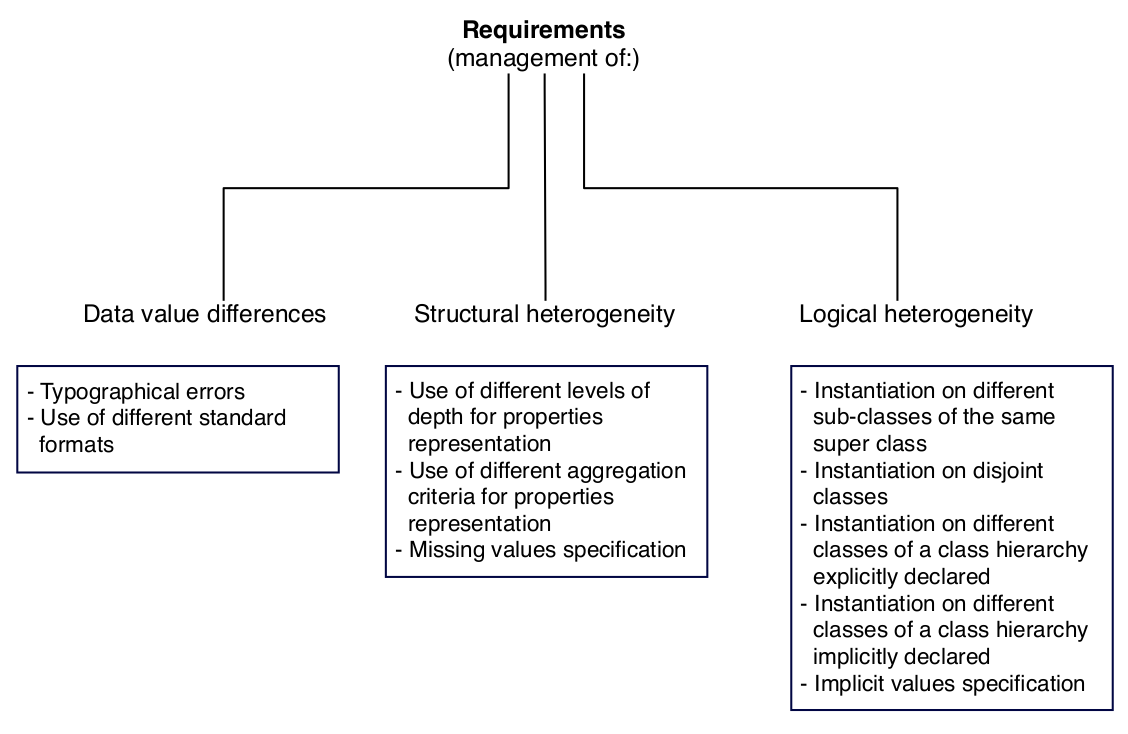
\includegraphics[width=0.9\textwidth]{./imagens/IMRequirements.png}
	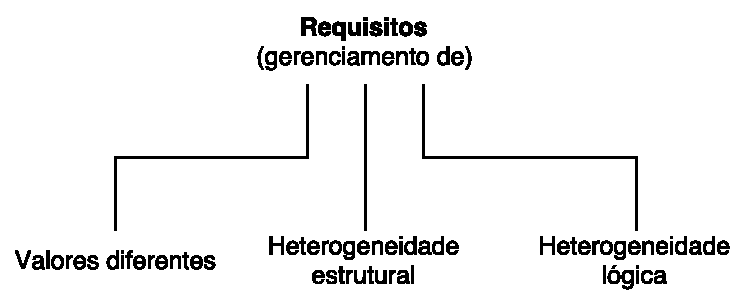
\includegraphics[width=0.9\textwidth]{./imagens/im_requirements.pdf}
    \caption{Requisitos para soluções de alinhamento de dados}
	\footnotesize{Fonte: baseado em \cite{ferrara2008towards}}
	\label{fig:imrequirements}
\end{figure}

\textbf{Valores diferentes:}
% * <profsean@gmail.com> 2017-01-18T20:15:13.295Z:
% 
% > Diferença de Valores:
% "Diferença de valores" (como está no texto) ou "Valores diferentes" (como está na figura)?
% 
% ^ <armandobs14@gmail.com> 2017-01-18T20:17:47.903Z:
%
% Ajustei para deixar de acordo com a imagem.
%
% ^ <armandobs14@gmail.com> 2017-01-18T20:17:50.727Z.
Um algoritmo de correspondência de instância deve reconhecer valores correspondentes, sempre que possível, mesmo quando esses valores possuem erros. Para mitigar esse problema, a comunidade utiliza abordagens como algoritmos de similaridade e transformação de valores.


\textbf{Heterogeneidade Estrutural:}
Instâncias que pertencem a ontologias diferentes diferem não somente entre propriedades e valores, mas também na sua estrutura. Desta forma, algoritmos de alinhamento de dados devem identificar propriedades semelhantes em ambos os recursos.


\textbf{Heterogeneidade Lógica:}
% * <profsean@gmail.com> 2017-01-18T20:18:47.062Z:
% 
% > Heterogeneidade Lógica:
% Não explicou...
% 
% ^ <armandobs14@gmail.com> 2017-01-18T20:36:14.777Z:
%
% O autor não descreve o que seria de fato a heterogeneidade lógica, dessa forma descrevi de acordo o meu entendimento.
%
% ^ <armandobs14@gmail.com> 2017-01-18T20:36:21.108Z.
A heterogeneidade lógica trata-se de um problema de alinhamento de ontologias, o qual não é levado em consideração no processo de alinhamento de dados, no entanto, faz-se necessário em tarefas de inferência. Esse problema diz respeito à semântica atribuída aos termos, havendo situações em que o mesmo termo pode ter significados diferentes atribuídos a ele (\textit{e.g.} manga - fruta e manga - vestimenta).

Diante do exposto, a comunidade vem desenvolvendo alternativas para a identificação de correspondência de instâncias. Diante disso, a seção a seguir apresenta os trabalhos relacionados a esta proposta.
% * <armandobs14@gmail.com> 2017-01-18T21:47:58.426Z:
% 
% > Diante do exposto, a comunidade vem desenvolvendo alternativas para a aperfeiçoar as soluções para a correspondência de instâncias . Diante disso, a seção aseguir apresenta trabalhos relacionado a esta proposta.
% 
% Melhorar a conexão entre os parágrafos.
% 
% ^ <armandobs14@gmail.com> 2017-01-19T01:07:55.371Z.

\section{Trabalhos Relacionados}
% * <profsean@gmail.com> 2017-01-18T20:19:34.451Z:
% 
% > Trabalhos
% Independente de juntar ou não os capítulos, é importante encadear esta parte do texto com a anterior... Ficou uma quebra... muda completamente de assunto...
% 
% ^ <armandobs14@gmail.com> 2017-01-19T01:08:23.836Z:
%
% Adicionei um parágrado ao final do capítulo anterior.
%
% ^ <armandobs14@gmail.com> 2017-01-19T01:08:25.949Z.
\label{cap:relacionados}
Neste capítulo serão apresentadas duas ferramentas para o alinhamento de dados conectados. As ferramentas apresentadas a seguir foram selecionadas  devido ao seu destaque na edição de 2016 do relatório publicado pela Ontology Alignment Evaluation Initiative (OAEI), mais especificamente na trilha referente à correspondência de instâncias (\textit{Instance Matching}). Inicialmente, a OAEI avaliava apenas ferramentas de alinhamento de ontologias, dando início à avaliação de soluções para alinhar dados em 2009. Desde então, um número crescente aplicações vêm sendo submetidas \cite{cheatham2015results}.
% * <profsean@gmail.com> 2017-01-18T20:22:17.708Z:
% 
% > Desde então, um número crescente aplicações vêm sendo submetidas
% Dados que comprovem? Evidências disto?
% 
% ^ <armandobs14@gmail.com> 2017-01-18T20:46:12.594Z:
%
% Citei o mesmo paper que utilizei na introdução.
%
% ^ <armandobs14@gmail.com> 2017-01-19T01:08:32.597Z.
% * <profsean@gmail.com> 2017-01-18T20:21:19.611Z:
% 
% > devido ao seu destaque
% Deveria explicar melhor que destaque foi esse... Preocupa o fato de ter considerado apenas 2 (e a escolha não estar bem clara)... também não sei se outras ferramentas com características mais próximas não deveriam ter sido consideradas (baseadas em instâncias)...
% 
% ^ <armandobs14@gmail.com> 2017-01-18T20:51:26.403Z:
%
% Citei que dentro do OAEI, essas ferramentas foram submetidas para a track de instance matching.
%
% ^ <armandobs14@gmail.com> 2017-01-19T01:10:08.818Z.

\subsection{AgreementMakerLight (AML)}
Desenvolvido em parceria entre o Instituto Gulbenkian de Ciência, a Universidade de Lisboa, e a Universidade de Illinois, o AgreementMakerLight é uma ferramenta de alinhamento de ontologias. De acordo com \cite{fariaoaei}, o AML se baseia inicialmente em técnicas e similaridade léxica, tendo como ênfase o uso de fontes externas como \textit{background}.

O AML conta com três algoritmos para alinhamento voltados a correspondência de instâncias, sendo eles o \textit{HybridStringMatcher}, o \textit{ValueStringMatcher} e o \textit{Value2LexiconMatcher}. O primeiro utiliza diversas abordagens para gerar a similaridade, sendo elas a comparação entre frases, palavras. Além disso, essa abordagem hibrida também explora a \textit{WordNet}. O segundo utiliza o mapeamento de valor para gerar calcular a similaridade, penalizando pares nos quais anotações ou propriedades de dados não são os mesmos. Por fim, o terceiro une as duas abordagens anteriores.

Apesar do AML possuir diferentes algoritmos de alinhamento na ferramenta, todos eles trabalham apenas no nível dos dados. Consequentemente, as características das propriedades são desconsideradas ao longo do processo de correspondência.

\subsection{RiMOM-2016}
Baseando-se no RiMOM  \cite{li2009rimom}, \citeonline{zhang2016rimom} desenvolveram o RiMOM-2016, que é uma ferramenta para alinhar dados conectados. Ela implementa um número considerável de abordagens para alinhar, cuja escolha é realizada através dos metadados extraídos da ontologia. Além disso, o RiMOM-2016 utiliza um índice invertido para indexar os objetos e consequentemente gerar pares candidatos para um possível alinhamento. A geração dos pares é realizada quando dois recursos compartilham pelo menos um predicado e objeto.

\begin{figure}[!ht]
	\centering
	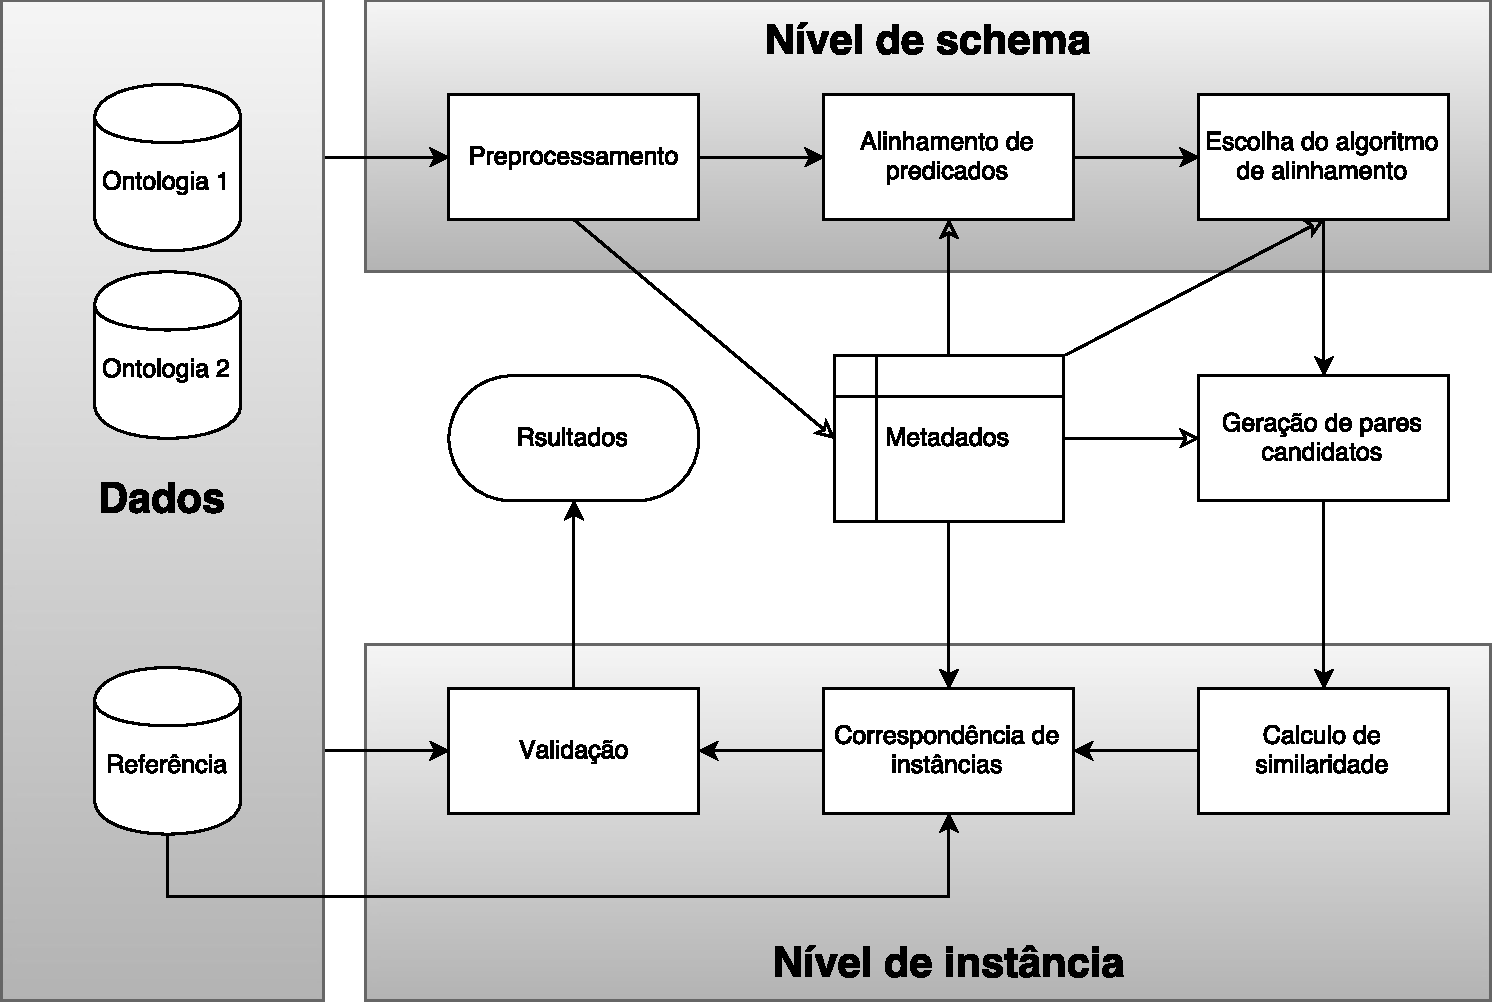
\includegraphics[width=0.8\textwidth]{./imagens/rimom_2016.pdf}
    \caption{Arquitetura do RiMOM-2016}
	\footnotesize{Fonte: adaptado de \cite{zhang2016rimom}}
	\label{fig:rimom}
\end{figure}

Por um lado, o índice invertido permite que um número menor de comparações seja realizado. Por outro lado, a etapa de construção desse índice não considera que os objetos indexados podem conter qualquer tipo de erro. Além disso, como pode ser visto na Figura \ref{fig:rimom}, o RiMOM-2016 utiliza as ontologias apenas para alinhar as propriedades e como entrada para a geração de metadados.

\subsection{Comparação com a proposta}

Neste capítulo, algumas das principais ferramentas existentes foram apresentadas. Essas ferramentas tem o objetivo de alinhar dados conectados através de diversas abordagens. Dentre os sistemas apresentados, nenhum deles contempla o alinhamento de dados como foco principal, sendo variações de ferramentas existentes para o alinhamento de ontologias.
% * <profsean@gmail.com> 2017-01-18T20:34:14.738Z:
% 
% > nenhum deles contempla o alinhamento de dados como foco principal
% Não tem nenhuma? Será que vc pesquisou direito? Será que não deveria ter buscado ferramentas que fazem alinhamento baseado em instâncias? Se não me engano o pessoal do Marco Antonio Casanova, prof. da PUC-Rio estava trabalhando com isso... não sei se deixaram ferramentas disponíveis. Sugiro dar uma pesquisada porque o Bernardo (que estará na sua banca) foi aluno do Casanova...
% 
% ^ <armandobs14@gmail.com> 2017-01-18T20:44:36.267Z:
%
% Nesse caso, quis dizer que nenhuma das ferramentas apresentadas tem o alinhamento de dados como foco principal, pois são adaptações de soluções para o alinhamento de ontologias.
%
% ^ <armandobs14@gmail.com> 2017-01-19T01:11:11.956Z.

Esta seção tem o objetivo de apresentar um comparativo entre os trabalhos relacionados e o presente estudo. Para isso, consideramos os seguintes critérios: 
\begin{enumerate}
\item \textbf{Quantidade de \textit{datasets} suportados:} Este critério refere-se à quantidade de de \textit{datasets} que podem ser utilizados para no processo de correspondência de instâncias. Normalmente, apenas dois \textit{datasets} são suportados simultaneamente. Com isso, a troca de um dos \textit{datasets} é necessária.
\item \textbf{Tipo de suporte à ontologia:} Este critério refere-se à maneira como as ontologias são exploradas pela ferramenta de correspondência de instâncias, podendo ser classificada como dirigida ou baseada em ontologia.  Uma ferramenta pode ser classificada como dirigida por ontologia quando explora a modelagem conceitual com o objetivo de escolher o conjunto de atividades que são utilizados no processo. Por outro lado, uma ferramenta é dita baseada em ontologias quando a modelagem conceitual é a base para o processo de correspondência.
\item \textbf{Utilização de computação específica:} Este critério refere-se à utilização de algoritmos específicos para os \textit{datasets} que serão utilizados no processo de correspondência de instâncias com o objetivo de melhorar a precisão das correspondências estabelecidas.
\item \textbf{Exploração dos conceitos presentes na ontologia:} Este critério refere-se a exploração dos conceitos presentes na modelagem conceitual. Além disso, as características dos relacionamentos são consideradas (\textit{e.g.} transividade).
\end{enumerate}

\begin{table}[h]
	\centering
	\caption{Comparação entre os trabalhos}
	\label{tab:comparacao}
	\begin{tabular}{@{}llll}
		\toprule
		\textbf{Critérios de comparação}                    & \textbf{RiMOM} & \textbf{AML} & \textbf{Proposta} \\ \midrule
		(1) Quantidade de \textit{datasets} suportados    & 2              & 2            & 2+                \\
% * <profsean@gmail.com> 2017-01-18T20:40:50.085Z:
% 
% > Quantidade de \textit{datasets} suportados
% Por que os dois só consideram 2 datasets? Você quer dizer no alinhamento consideram 2 a 2 entidades?
% 
% ^ <armandobs14@gmail.com> 2017-01-18T20:55:00.624Z:
% 
% Eles são capazes de realizar a correspondência de dois datasets por vez (e.g. Lattes <-> SBIE). Dessa forma, para utilizar um outro dataset é necessário trocar um deles (e.g. Lattes <-> WIE). Já a proposta suporta mais de dois datasets por vez (e.g. Lattes <-> [SBIE,WIE,SBIE]).
% 
% ^ <armandobs14@gmail.com> 2017-01-19T01:11:59.559Z.
		(2) Tipo de suporte à ontologia                     & Dirigido       & Dirigido     & Baseado           \\
% * <profsean@gmail.com> 2017-01-18T20:40:17.651Z:
% 
% > Tipo de suporte
% Isto deveria ter sido melhor explicado... o que quer dizer? O que é dirigido e baseado?
% 
% ^ <armandobs14@gmail.com> 2017-01-19T01:12:16.222Z.
		(3) Utilização de computação específica             & Sim            & Sim          & Não               \\
		(4) Exploração dos conceitos presentes na ontologia & Não            & Não          & Sim               \\ \bottomrule
	\end{tabular}
\end{table}

Contudo, apesar das ferramentas se mostrarem capazes de encontrar correspondência entre instâncias, ainda deixam a desejar em alguns critérios, tais como a utilização de computação específica para os \textit{datasets}, além da pouca exploração das ontologia, que são utilizadas apenas para a geração de metadados, com o objetivo de escolher entre as abordagens de correspondência disponíveis. Diferentemente das ferramentas citadas, a proposta utiliza ontologias para guiar o processo de correspondência de instância. Além disso, essa abordagem permite que o usuário defina como o alinhamento deve ser realizado.

Outro diferencial da proposta em relação aos trabalhos relacionados está no que chamamos de alinhamento em cascata, que consiste na utilização de instâncias que pertencem a conceitos relacionados ao conceito cujas instâncias serão alinhadas.  O alinhamento em cascata vai além das instâncias, ele explora os relacionamentos existentes. A partir disso, é possível encontrar novas correspondências. Ademais, a proposta permite que as correspondências entre as instâncias sejam armazenadas diretamente na base de triplas (\textit{triple store}) em que estão armazenadas.
% * <profsean@gmail.com> 2017-01-18T20:43:43.697Z:
% 
% > alinhamento em cascata, que consiste na utilização de instâncias que pertencem a conceitos relacionados ao conceito cujas instâncias serão alinhadas.
% Isto deveria ser melhor explicado... Por que o alinhamento em cascata é importante? Como esta importância é percebida?
% 
% ^ <armandobs14@gmail.com> 2017-01-19T01:54:05.765Z.